
% Experement data + calcs goes here %

\section{Схема установки}

Схема установки представлена на рисунке 2.

\pic{0.8\linewidth}{scheme2.jpg}{Схема установки}

\newpage

\section{Ход работы}

\subsection{Вольт-амперная характеристика тиратрона в динамическом режиме}

Пронаблюдали ВАХ для двух различных напряжений лампы накала: \\

$ V\ruB{накала} = \left( 2,90 \pm 0,05 \right) \, $ В \\
$ V\ruB{накала} = \left( 2,65 \pm 0,05 \right) \, $ В \\

\begin{center}

\shiftedText{0cm}{0.4\linewidth}
{
    \begin{center}
        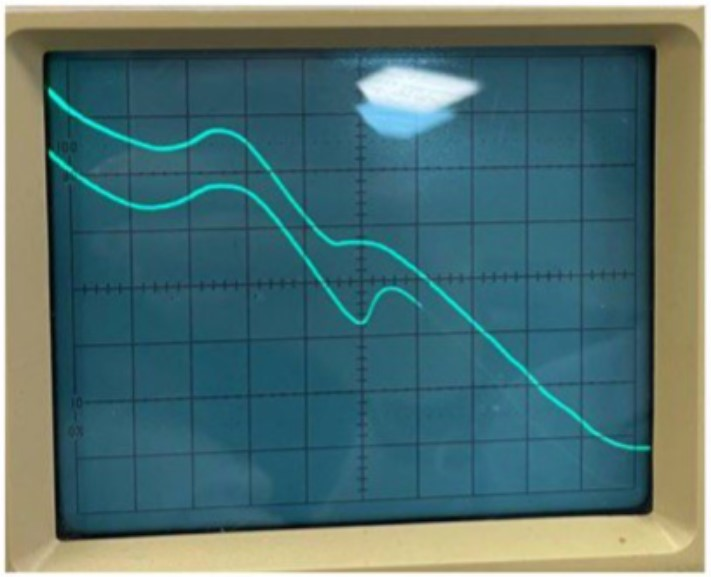
\includegraphics[width = \textwidth]{oscil1.jpg}
        \textit{Рис \arabic{PicsCounter}. ВАХ для $ 2,90 $ В}
    \end{center}

    \stepcounter{PicsCounter}
} \shiftedText{0cm}{0.4\linewidth}
{
    \begin{center}
        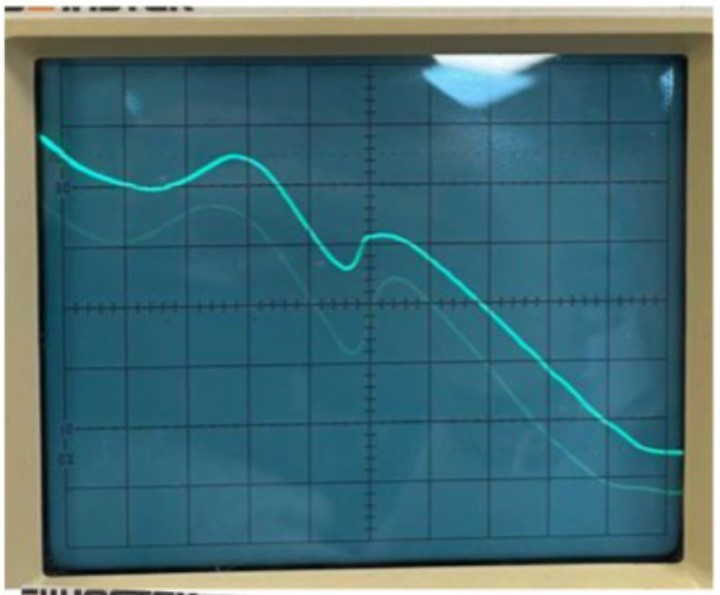
\includegraphics[width = \textwidth]{oscil2.jpg}
        \textit{Рис \arabic{PicsCounter}. ВАХ для $ 2,65 $ В}
    \end{center}

    \stepcounter{PicsCounter}
}

\end{center}

Получил напряжение пробоя для обоих значений $ V\ruB{накала} \, $:
$ \left( 11,0 \pm 0,5 \right) $ эВ и $ \left( 12,0 \pm 0,5 \right) $ эВ соответственно.
Достаточно большая величина погрешности обусловлена неполным совпадением графиков для
прямого и обратного хода характеристик.

\subsection{Вольт-амперная характеристика тиратрона в статическом режиме}

Произвели измерение ВАХ тиратрона для двух напряжений накала ($ 2,90 $ В и $ 2,65 $ В).
Собранные данные представлены в на рисунках 5 и 6.

\begin{center}

    \shiftedText{0cm}{0.4\linewidth}
    {
        \begin{center}
            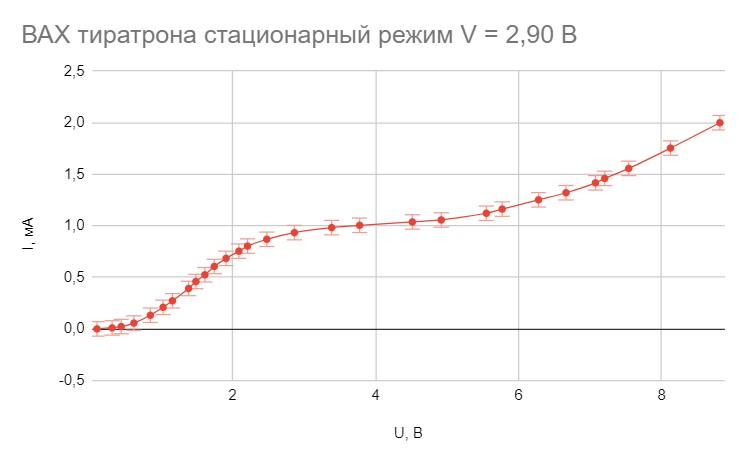
\includegraphics[width = \textwidth]{graph1.jpg}
            \textit{Рис \arabic{PicsCounter}. ВАХ для $ 2,90 $ В}
        \end{center}
    
        \stepcounter{PicsCounter}
    } \shiftedText{0cm}{0.4\linewidth}
    {
        \begin{center}
            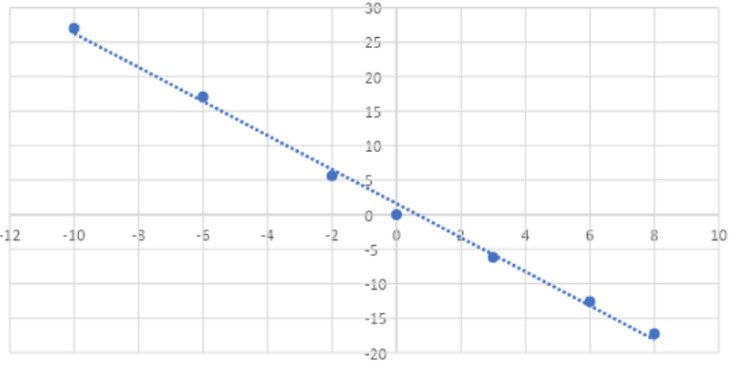
\includegraphics[width = \textwidth]{graph2.jpg}
            \textit{Рис \arabic{PicsCounter}. ВАХ для $ 2,65 $ В}
        \end{center}
    
        \stepcounter{PicsCounter}
    }
    
    \end{center}

\newpage{}

\subsection{Обработка результатов}

Расчеты погрешностей см. на листочке с расчетами.

\subsection{Вольт-амперная характеристика тиратрона в динамическом режиме}

Полученные значения для напряжения пробоя соответствуют табличному значению напряжения
пробоя для \textbf{ксенона}. \\

Снял значения с осфиллограммы:

Для $ 2,90 $ В: $ E_1 = \left( 2,0 \pm 0,2 \right) \, $ В и
$ E_1 = \left( 6,0 \pm 0,2 \right) \, $ В \\
Для $ 2,65 $ В: $ E_1 = \left( 1,6 \pm 0,2 \right) \, $ В и
$ E_1 = \left( 4,6 \pm 0,2 \right) \, $ В \\

Из формулы (\ref{EffectiveAtomSize}) получил эффективный размер атома:

l = $ \left( 3,7 \pm 0,2 \right) \cdot 10^{-10} \, $ м. \\

Так же посчитал $ U_0 $ по формуле (\ref{EffectivePotentialWellDepth}):

Для $ 2,90 $ В: $ U_0 = \left( 1,2 \pm 0,5 \right) \, $ В. \\
Для $ 2,65 $ В: $ U_0 = \left( 0,8 \pm 0,5 \right) \, $ В.

\subsection{Вольт-амперная характеристика тиратрона в статическом режиме}

Полученные в статическом режиме гарфики ВАХ не соответствуют как теоретической картине, так и
результатам, полученным в динамическом режиме.

Поэтому делать расчеты, связанные с этими значениями не имеет особого смысла.

\section{Вывод}

В ходе данной лабораторной работы хорошо показал себя динамический метод. А при
исследовании в статике, получились несогласующиеся с теорией и практикой данные. \\

Проблемы с динамическим методом могли возникнуть из-за достаточно сильной инертности и
нестабильности в работе лампы накаливания. В ходе работы напряжение на ней продолжало
достаточно существенно флуктуировать в течении более чем 30 минут после поворота
регулирующей ручки. \\

Данная особенность не повлияла на динамический метод, данные для которого снимаются
достаточно быстро. \\

Повысить точность измерений в статическом методе можно путем повышения стабильности работы
и скорости отклика лампы накаливания. \\

Повысить точность измерений в динамическом методе можно путем увеличения точности
шкалы осциллографа (все погрешности в динамическом методе обусловлены точностью снятия
напряжений с этой шкалы).
